\documentclass[landscape]{article}
\usepackage[pdftex]{graphicx}
\pagestyle{empty}
\oddsidemargin  -0.5 in
\evensidemargin -0.5 in
\headheight     0 in
\topmargin      -1 in
\textheight     7.7 in
\textwidth      10 in
\begin{document}
\huge
\renewcommand{\labelitemi}{-}
\setlength{\parindent}{0 cm}

\begin{figure}[!ht]
  \begin{center}
    \begin{tabular}{p{0.49\linewidth} p{0.49\linewidth}}
      \begin{minipage}{\linewidth} \begin{center} Electrons left-polarized 95\% \end{center} \end{minipage} &
      \begin{minipage}{\linewidth} \begin{center} Electrons right-polarized 95\% \end{center} \end{minipage} \\
      \begin{minipage}{\linewidth} 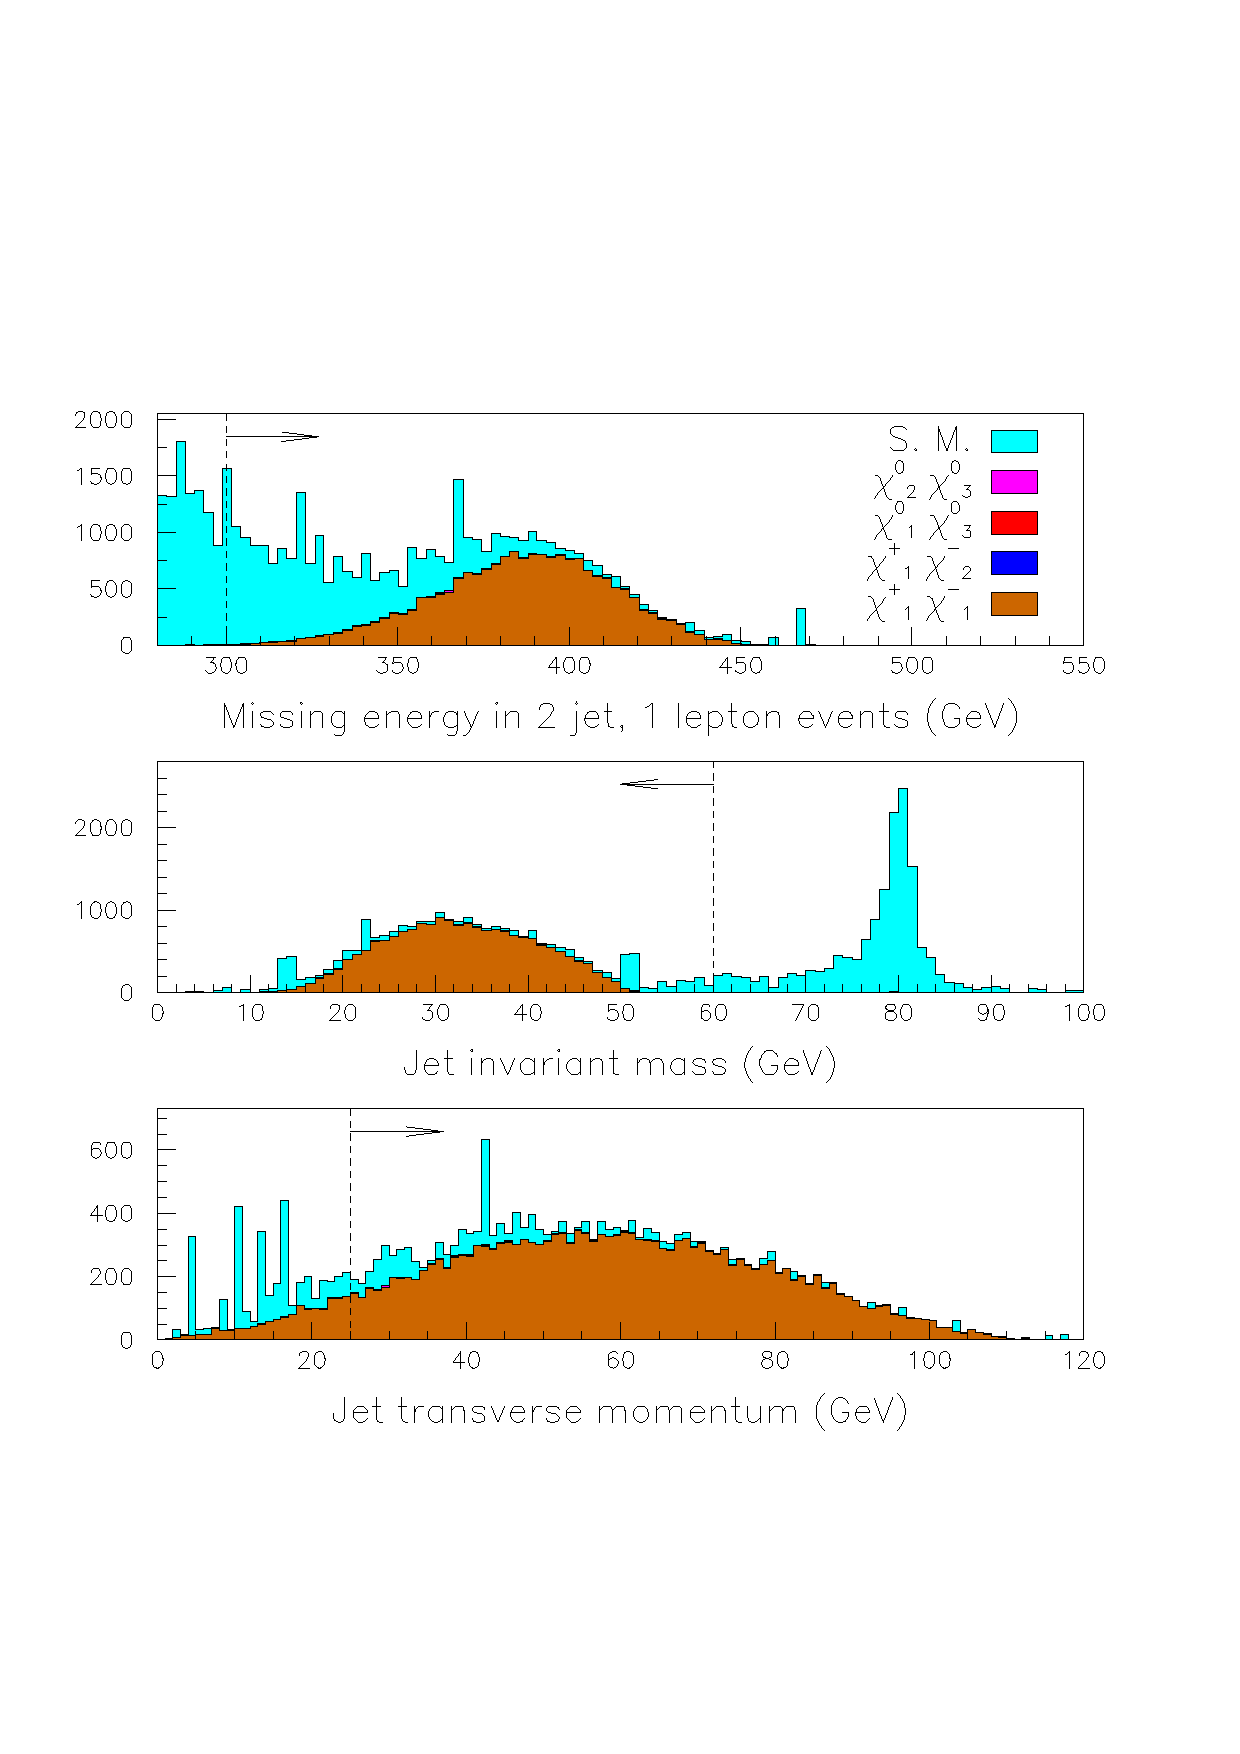
\includegraphics[width=\linewidth]{charginos_left.pdf} \end{minipage} &
      \begin{minipage}{\linewidth} \includegraphics[width=\linewidth]{charginos_right.pdf} \end{minipage}
    \end{tabular}

    \caption{\large Three cuts used to define $\chi_1^+\chi_1^-$ events, top
    to bottom: missing energy $>$ 300 GeV, di-jet invariant mass $<$
    60 GeV, and missing transverse jet momentum $>$ 25 GeV, applied
    cumulatively.  The plots on the left show 250 fb$^{-1}$ with
    electrons left-polarized, the ones on the right show 250 fb$^{-1}$
    with electrons right-polarized.  Brown is signal, light blue is
    all Standard Model background.  SUSY backgrounds are negligible
    for this mode.}

    \label{jimpcharginocuts}
  \end{center}
\end{figure}

What's different?  Jets and leptons must be within $|\cos\theta| <$
0.95.  My backgrounds are {\it not} two-photon; they are $e^+e^- \to
\ell^+\ell^- \nu \bar{\nu} Q \bar{Q}$ and $\to q \bar{q} b \bar{b} b
\bar{b}$ (where $q$ = $u$, $d$, $c$, $s$, and $Q$ = $u$, $d$, $c$,
$s$, $b$).

\pagebreak

Is that cut too loose?  Do jets at high angles have a distorted energy
spectrum because of lost particles?  (Compare generated jet energy
against reconstructed.)

\vfill

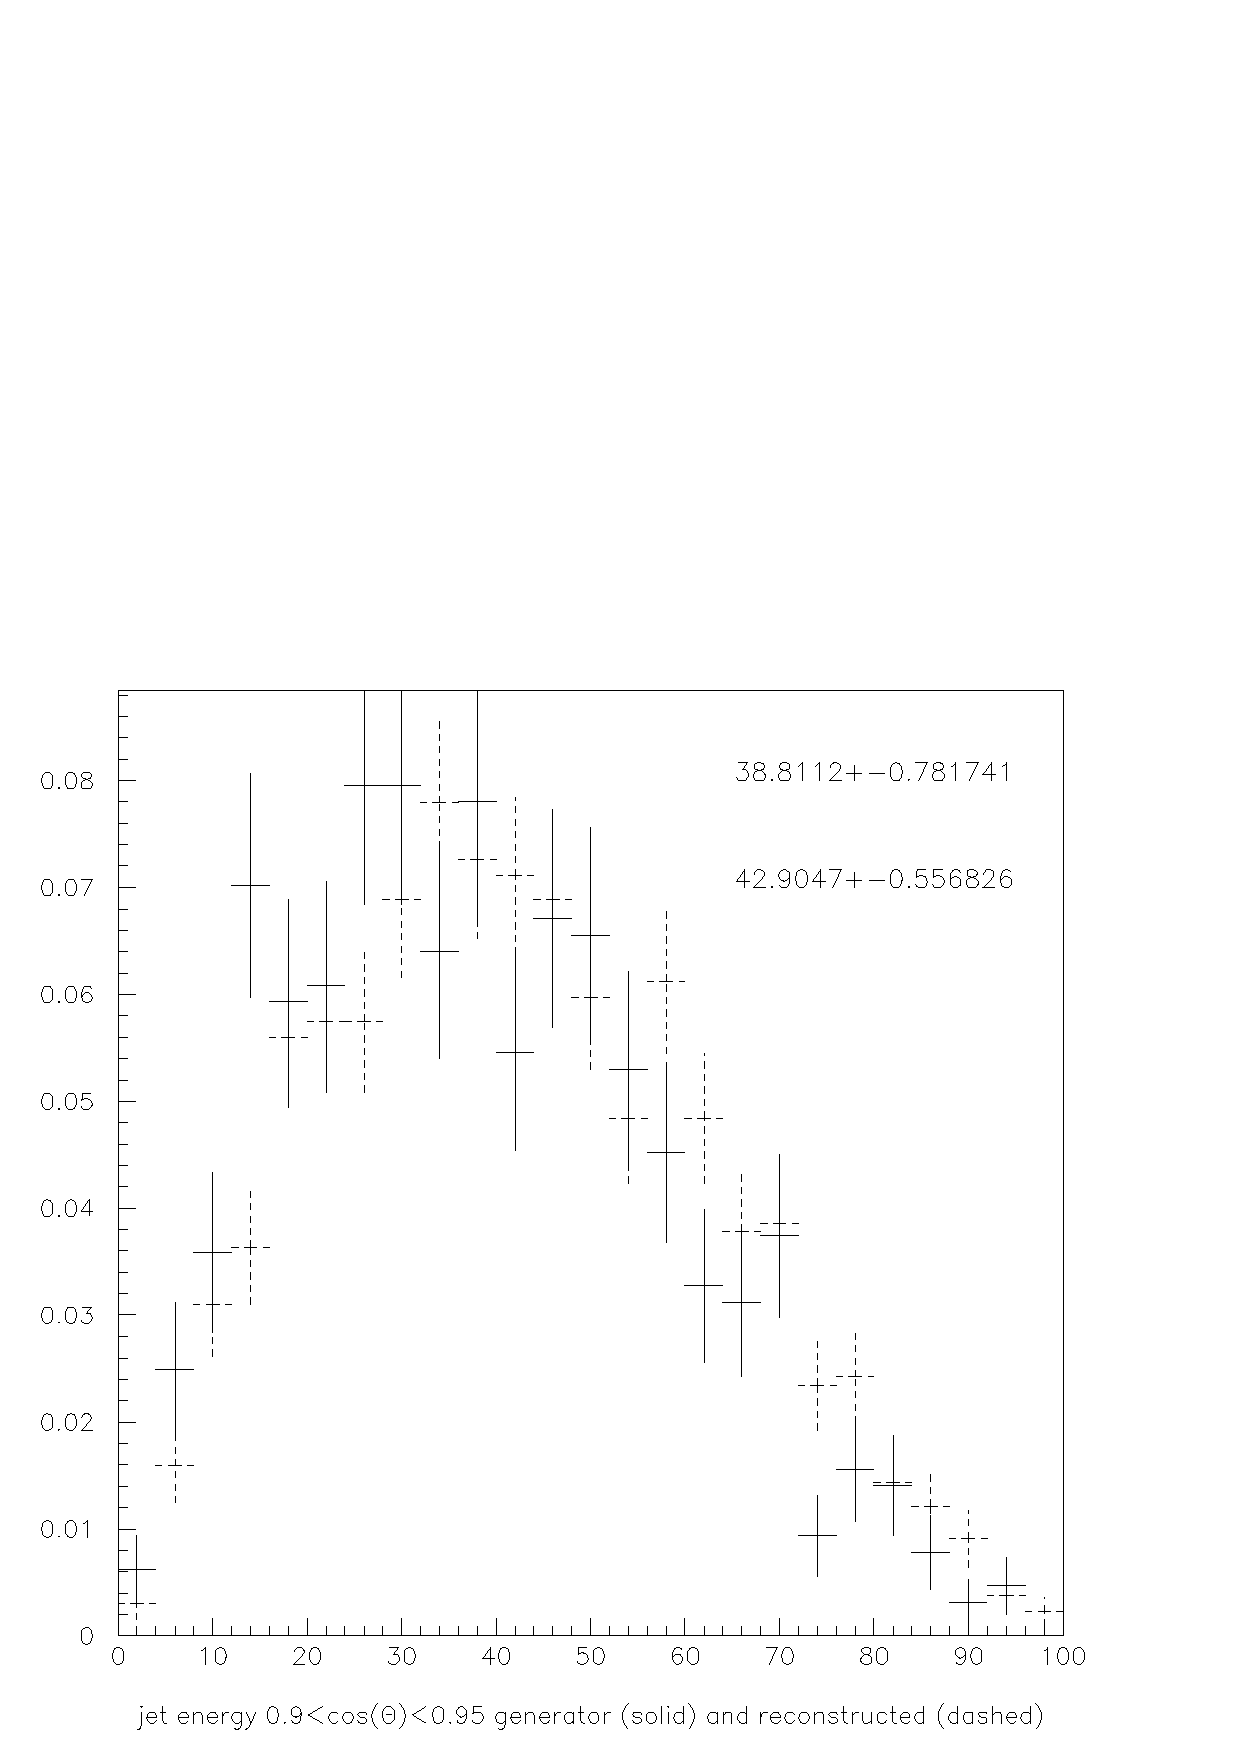
\includegraphics[width=0.7\linewidth]{high-angle_energy_distortion.pdf}

\pagebreak

Answer: not any more than the usual jet energy loss.

\vfill

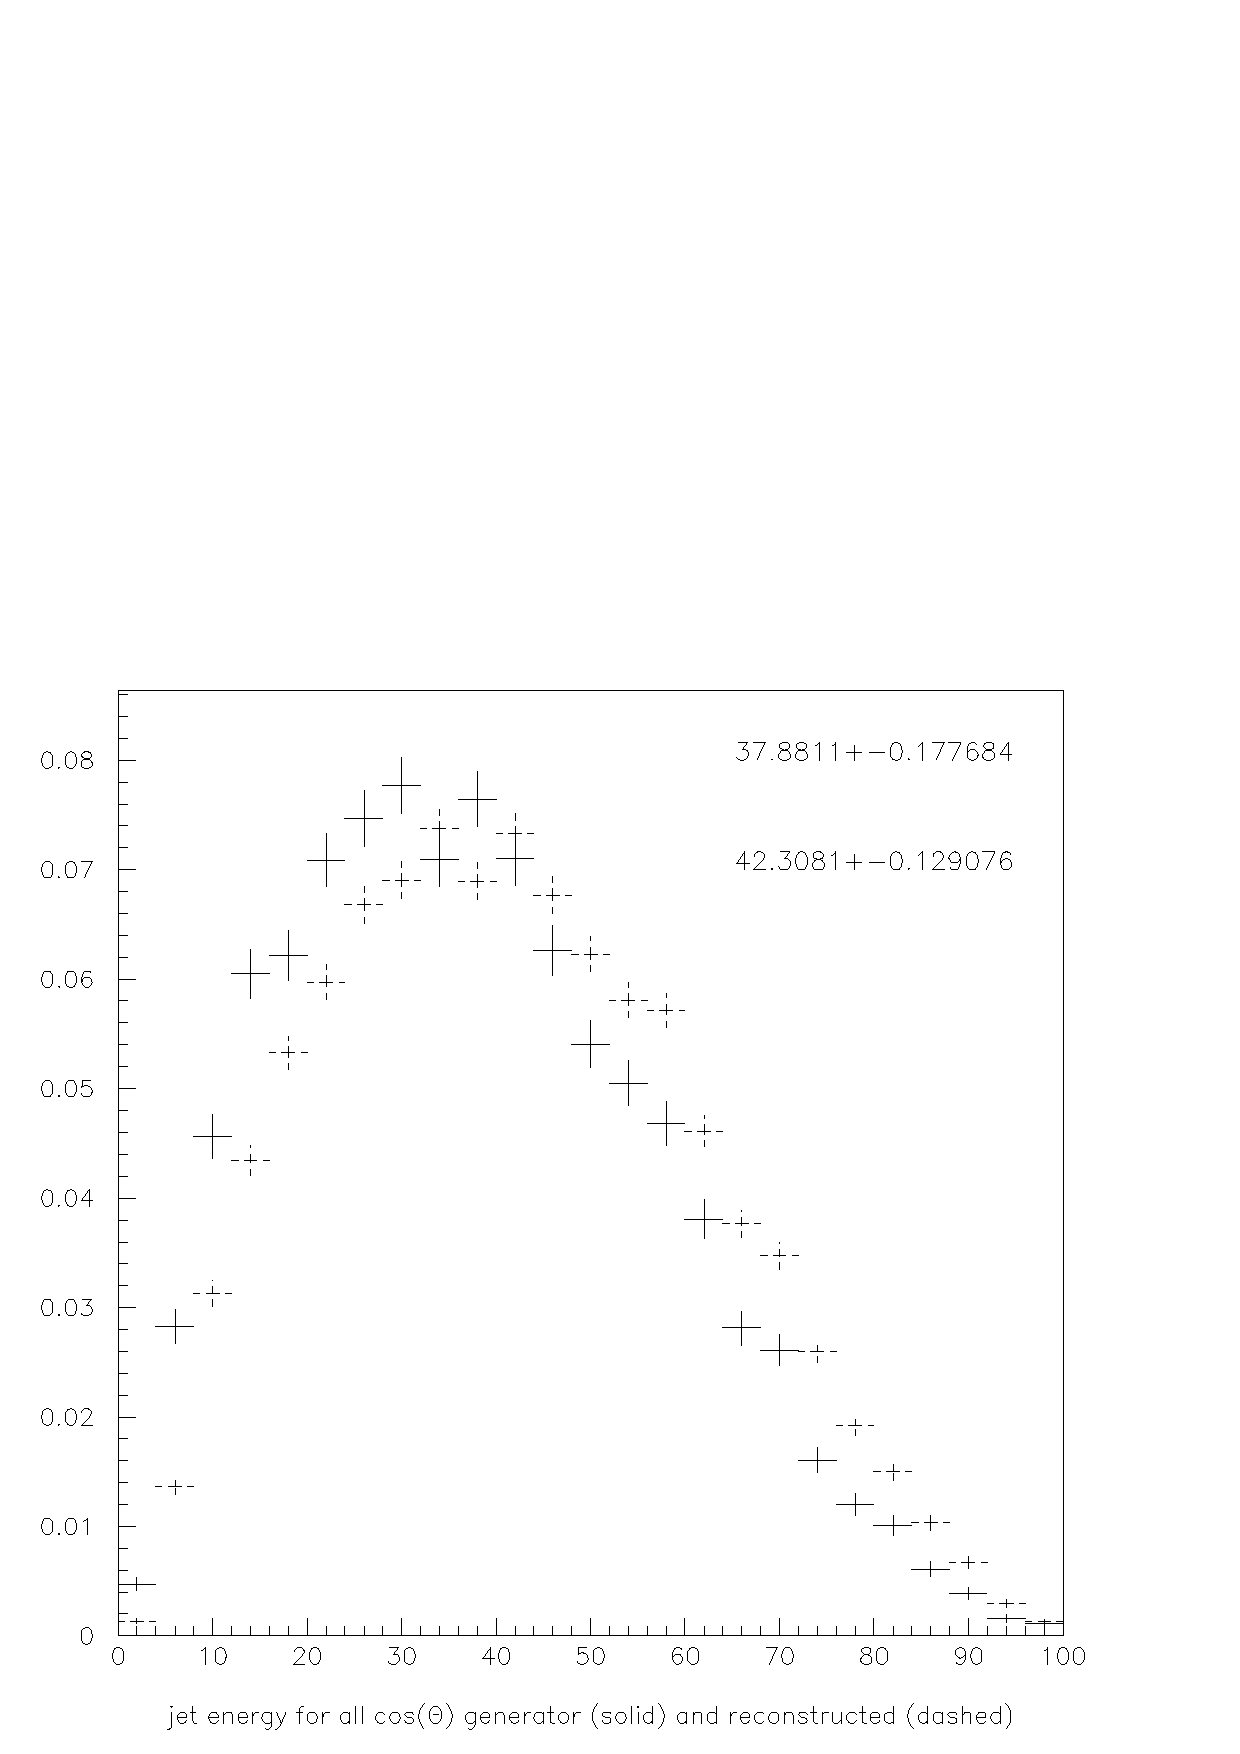
\includegraphics[width=0.7\linewidth]{high-angle_energy_distortion3.pdf}

\pagebreak

Are there efficiency losses when the jets come too close?  Looks like
more efficiency is lost when they're too far away?!?

\vfill

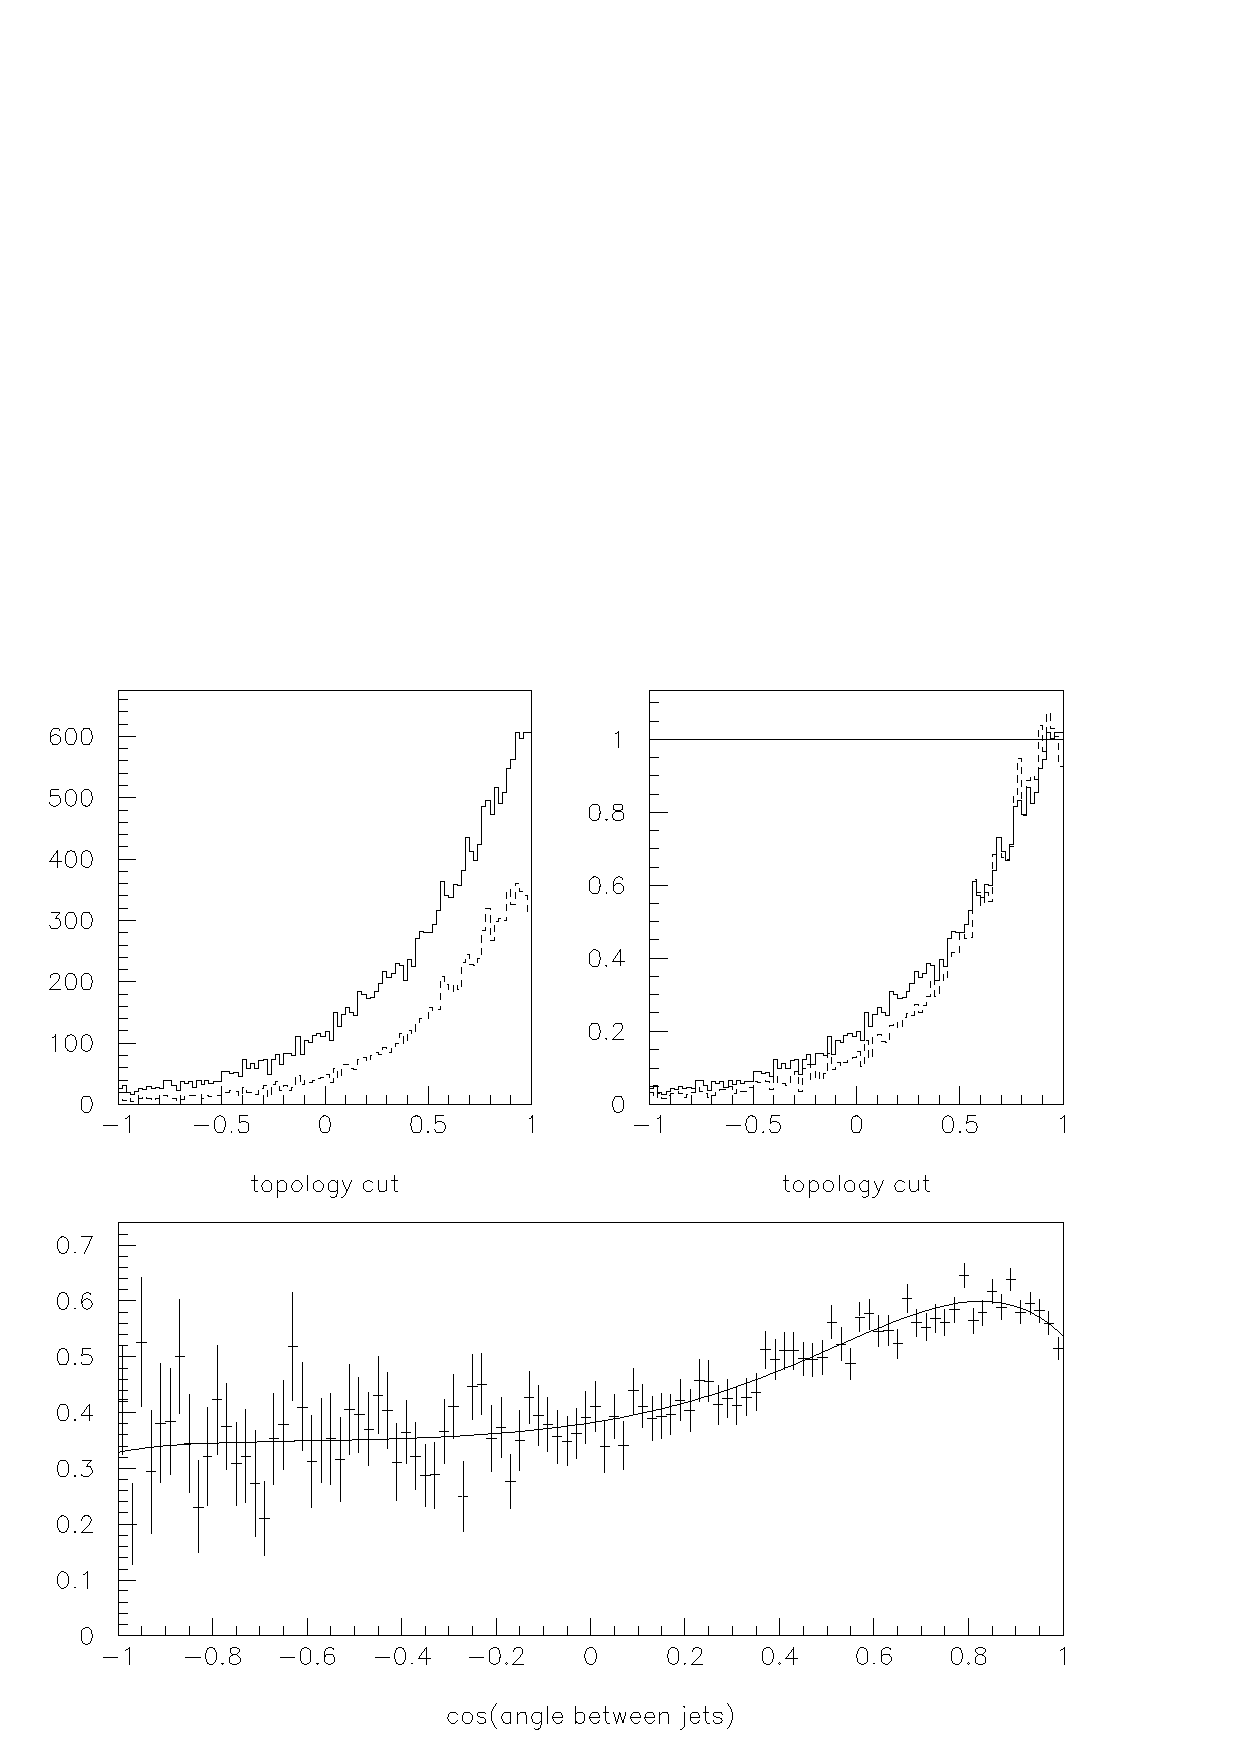
\includegraphics[width=0.7\linewidth]{jet_confusion1.pdf}

\pagebreak

Aha!  It's the isolated lepton cut that dominates efficiency losses.

\vfill

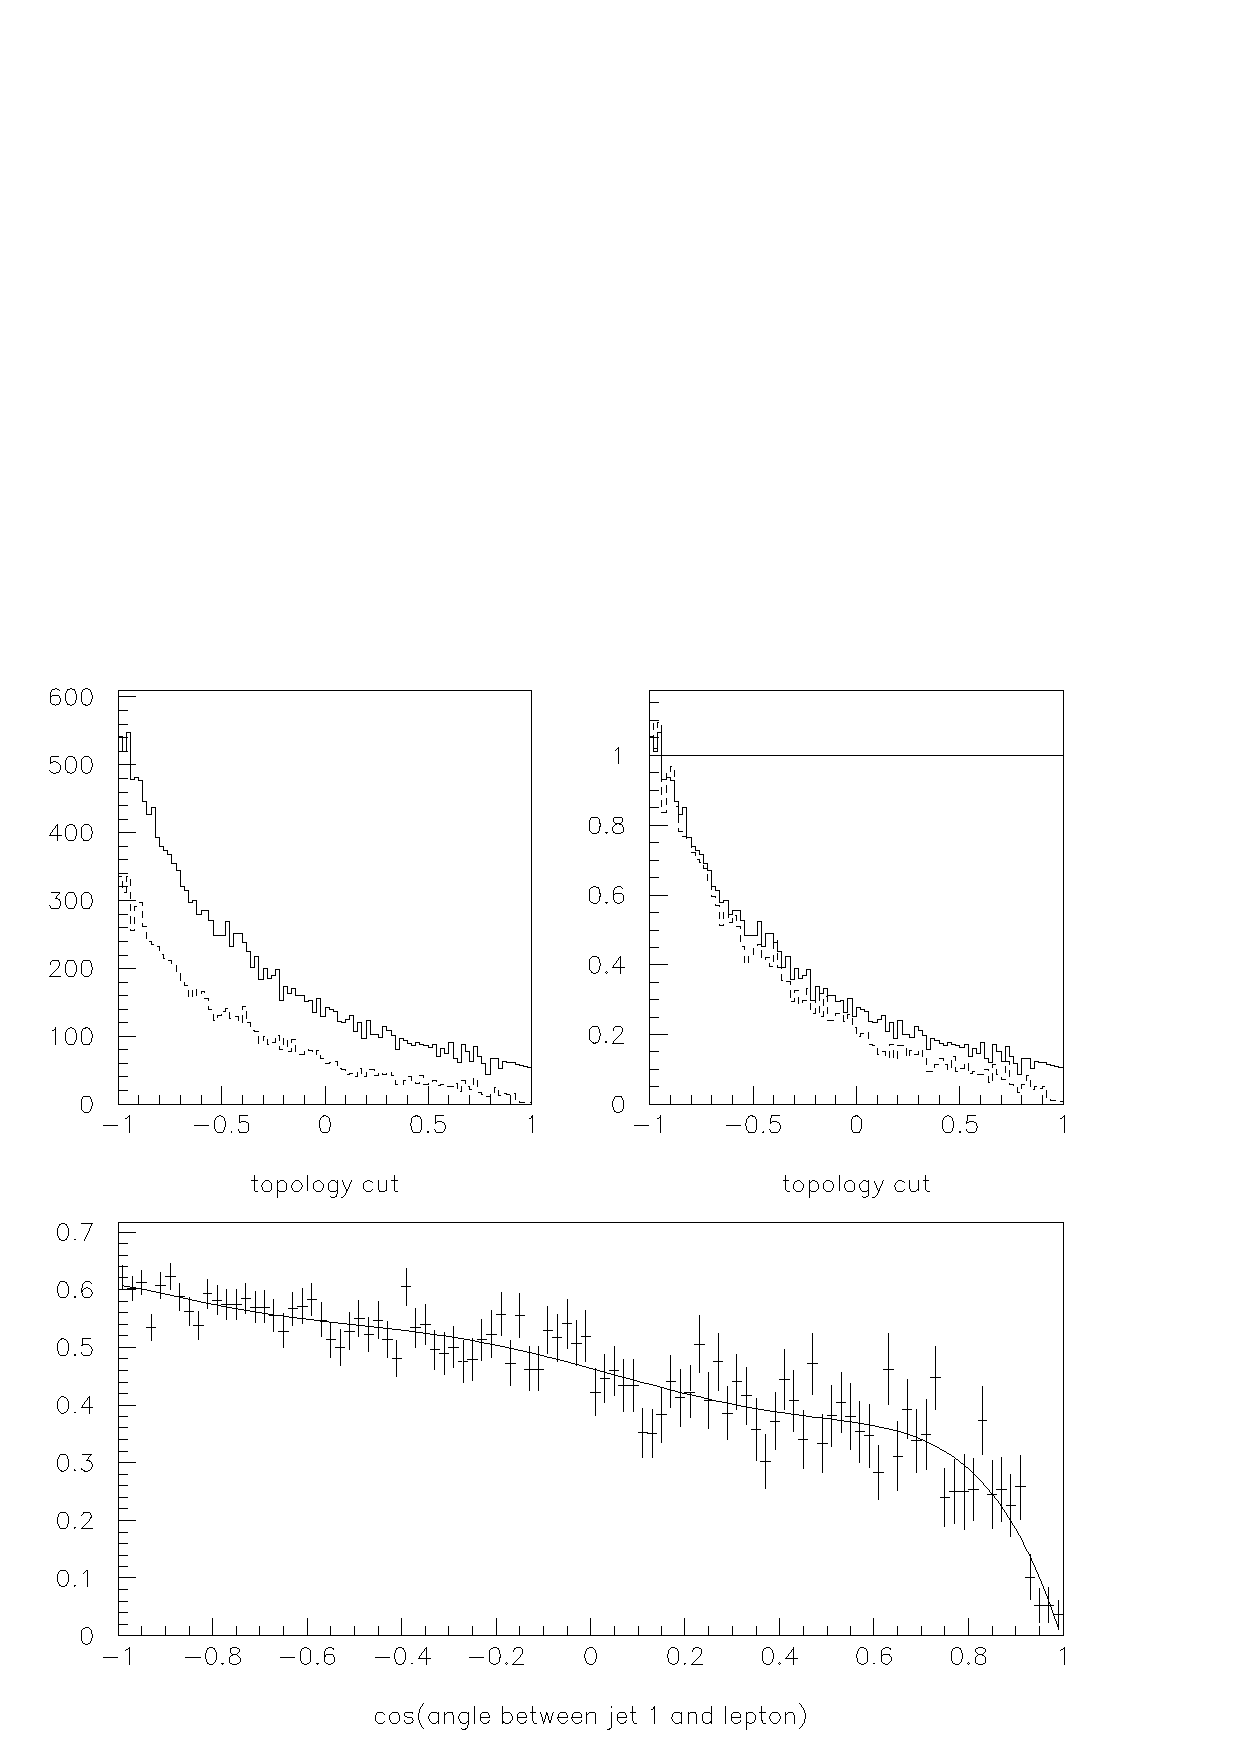
\includegraphics[width=0.7\linewidth]{jet_confusion2.pdf}

\pagebreak

To measure this effect: plot efficiency loss for when both jets are
the same specified angle from the lepton ($\pm$ 0.4).  Then
square-root this for the efficiency loss due to a single jet near the
lepton (so I can apply it to each jet independently).

\vfill

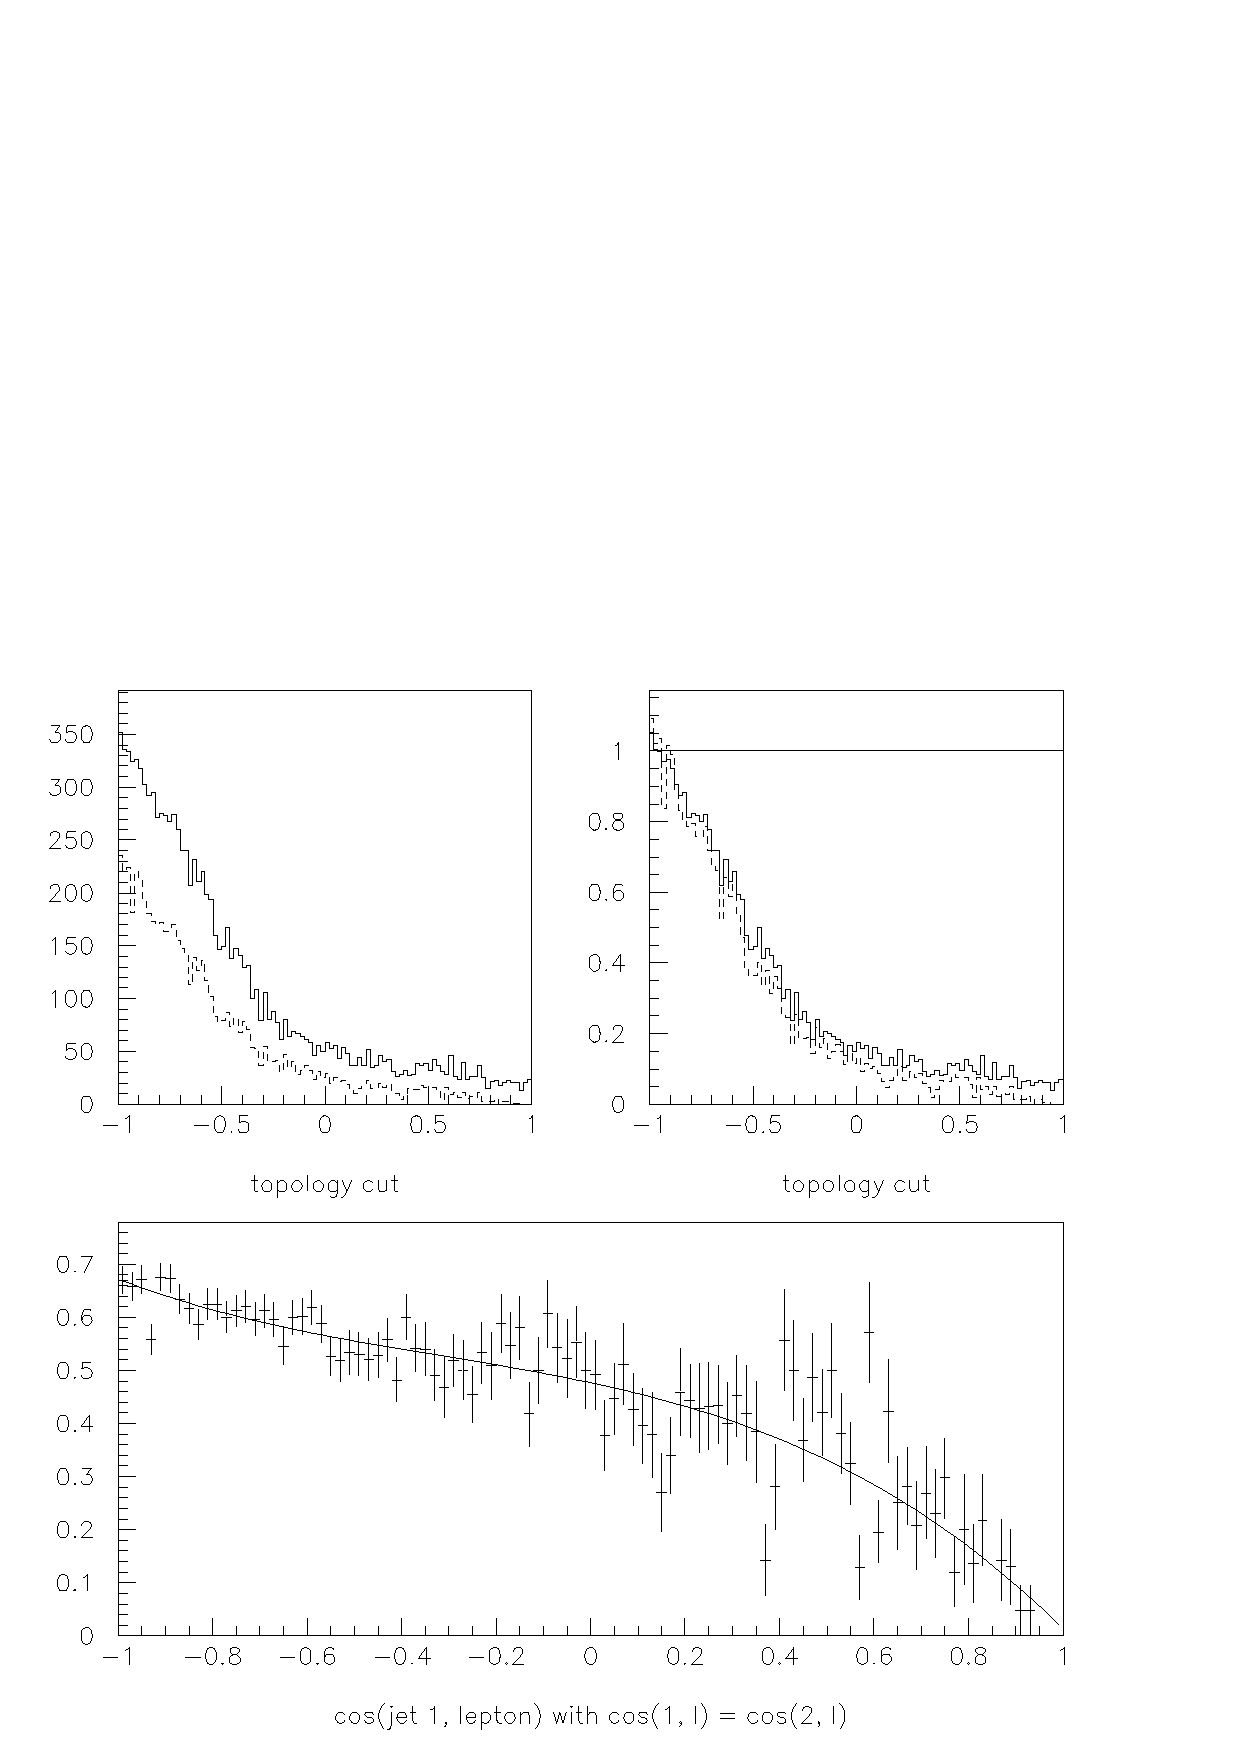
\includegraphics[width=0.65\linewidth]{jet_confusion4.pdf}

\pagebreak

Another effect: jet-jet invariant mass is not symmetrically smeared,
it's smeared in one direction: down.  This is an invariant mass plot
of our infinitely-narrow $Z^0$ peak in two jets--- there are no events
below zero.  Last bin is an overflow bin for the rest of the tail.

\vfill

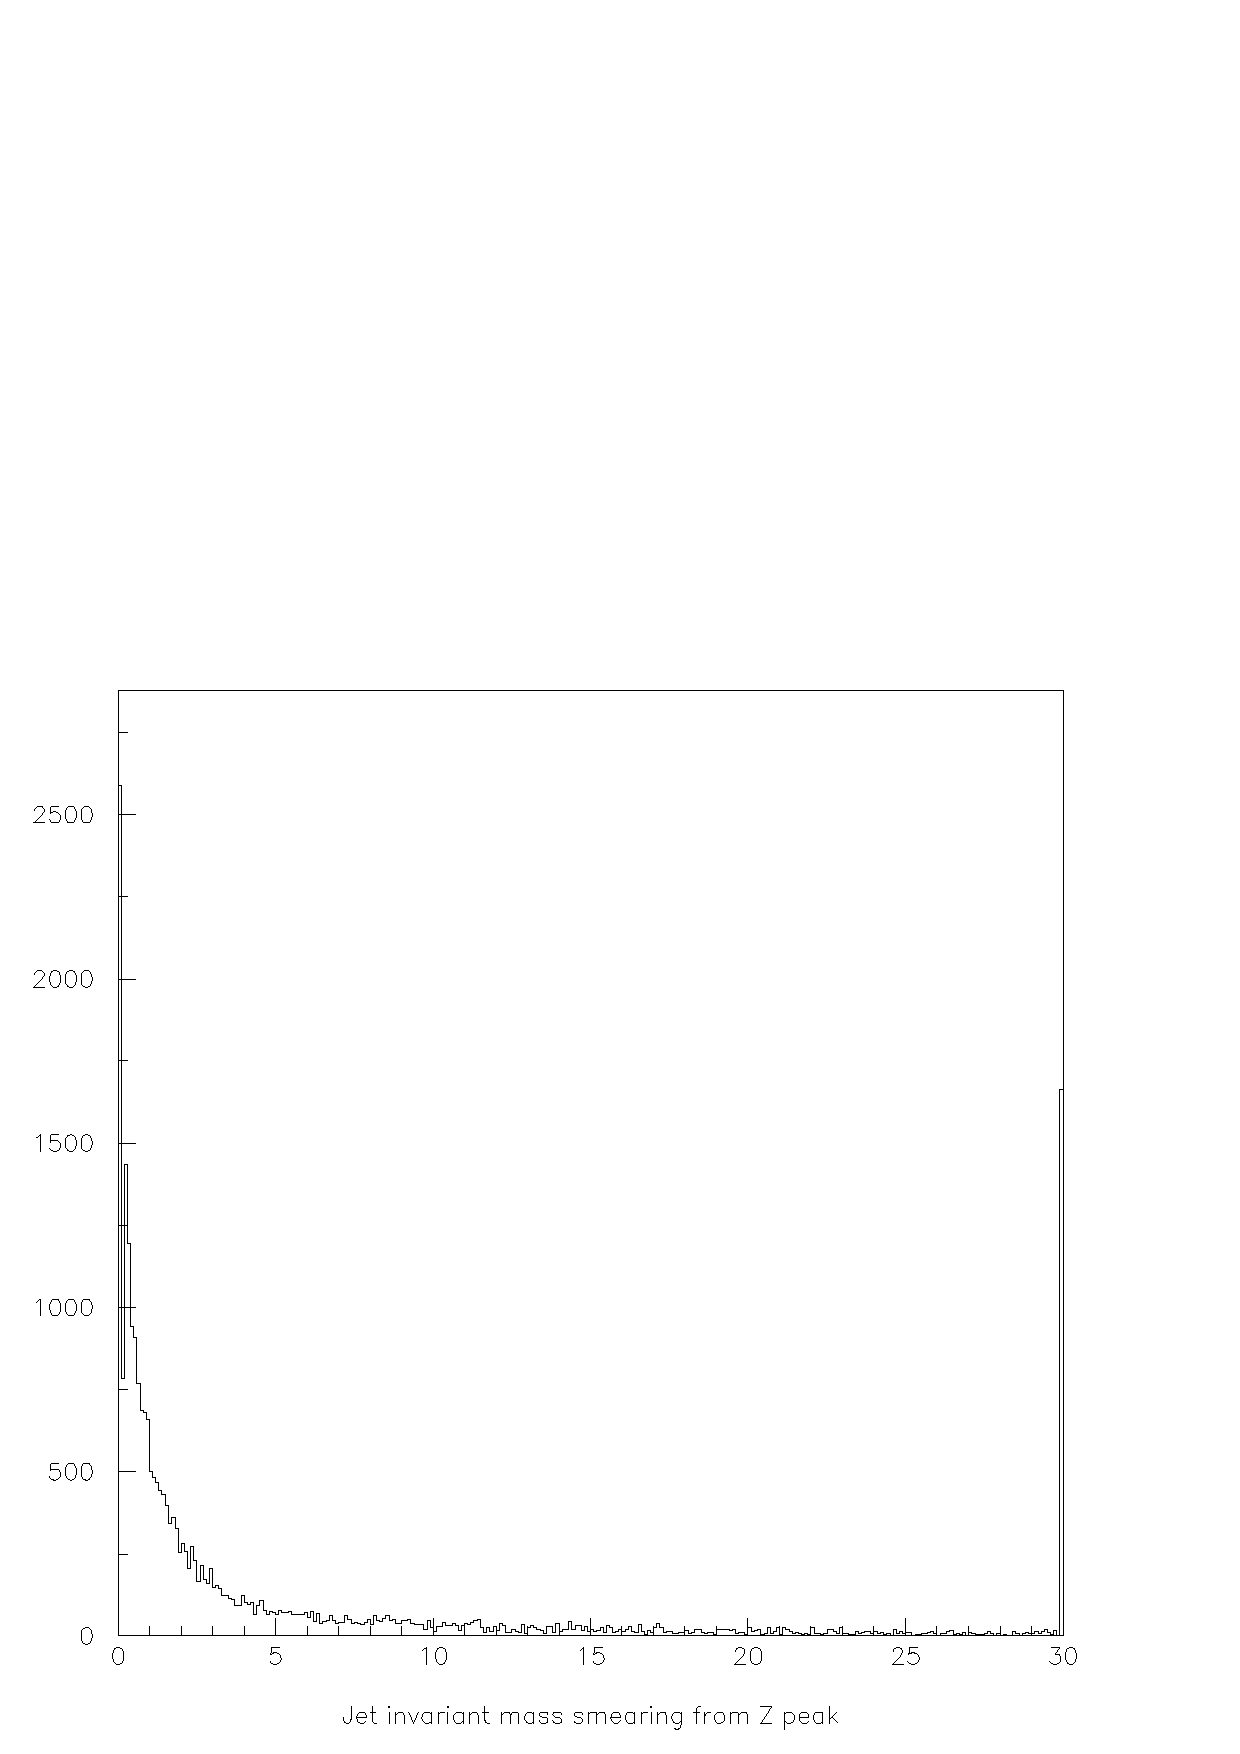
\includegraphics[width=0.65\linewidth]{z_smearing_with_overflow.pdf}

\pagebreak

What's in my simulation?

\begin{itemize}

\item Initial state radiation

\item All kinematics of decaying particles (including off-shell $W^\pm$ masses from Andreas's function)

\item Kinematic cuts that matter: $|\cos \theta| <$ 0.95 for jets and lepton, missing transverse jet momentum

\item Efficiency loss due to jet-confused lepton

\item Jet invariant mass smearing (from $Z^0$ jet invariant mass distribution)

\item Two-dimensional fit to jet-jet mass/total jet energy

\item Data has errors inflated by (completely unbiased) background subtraction

\end{itemize}

\pagebreak

What came out?

\vfill

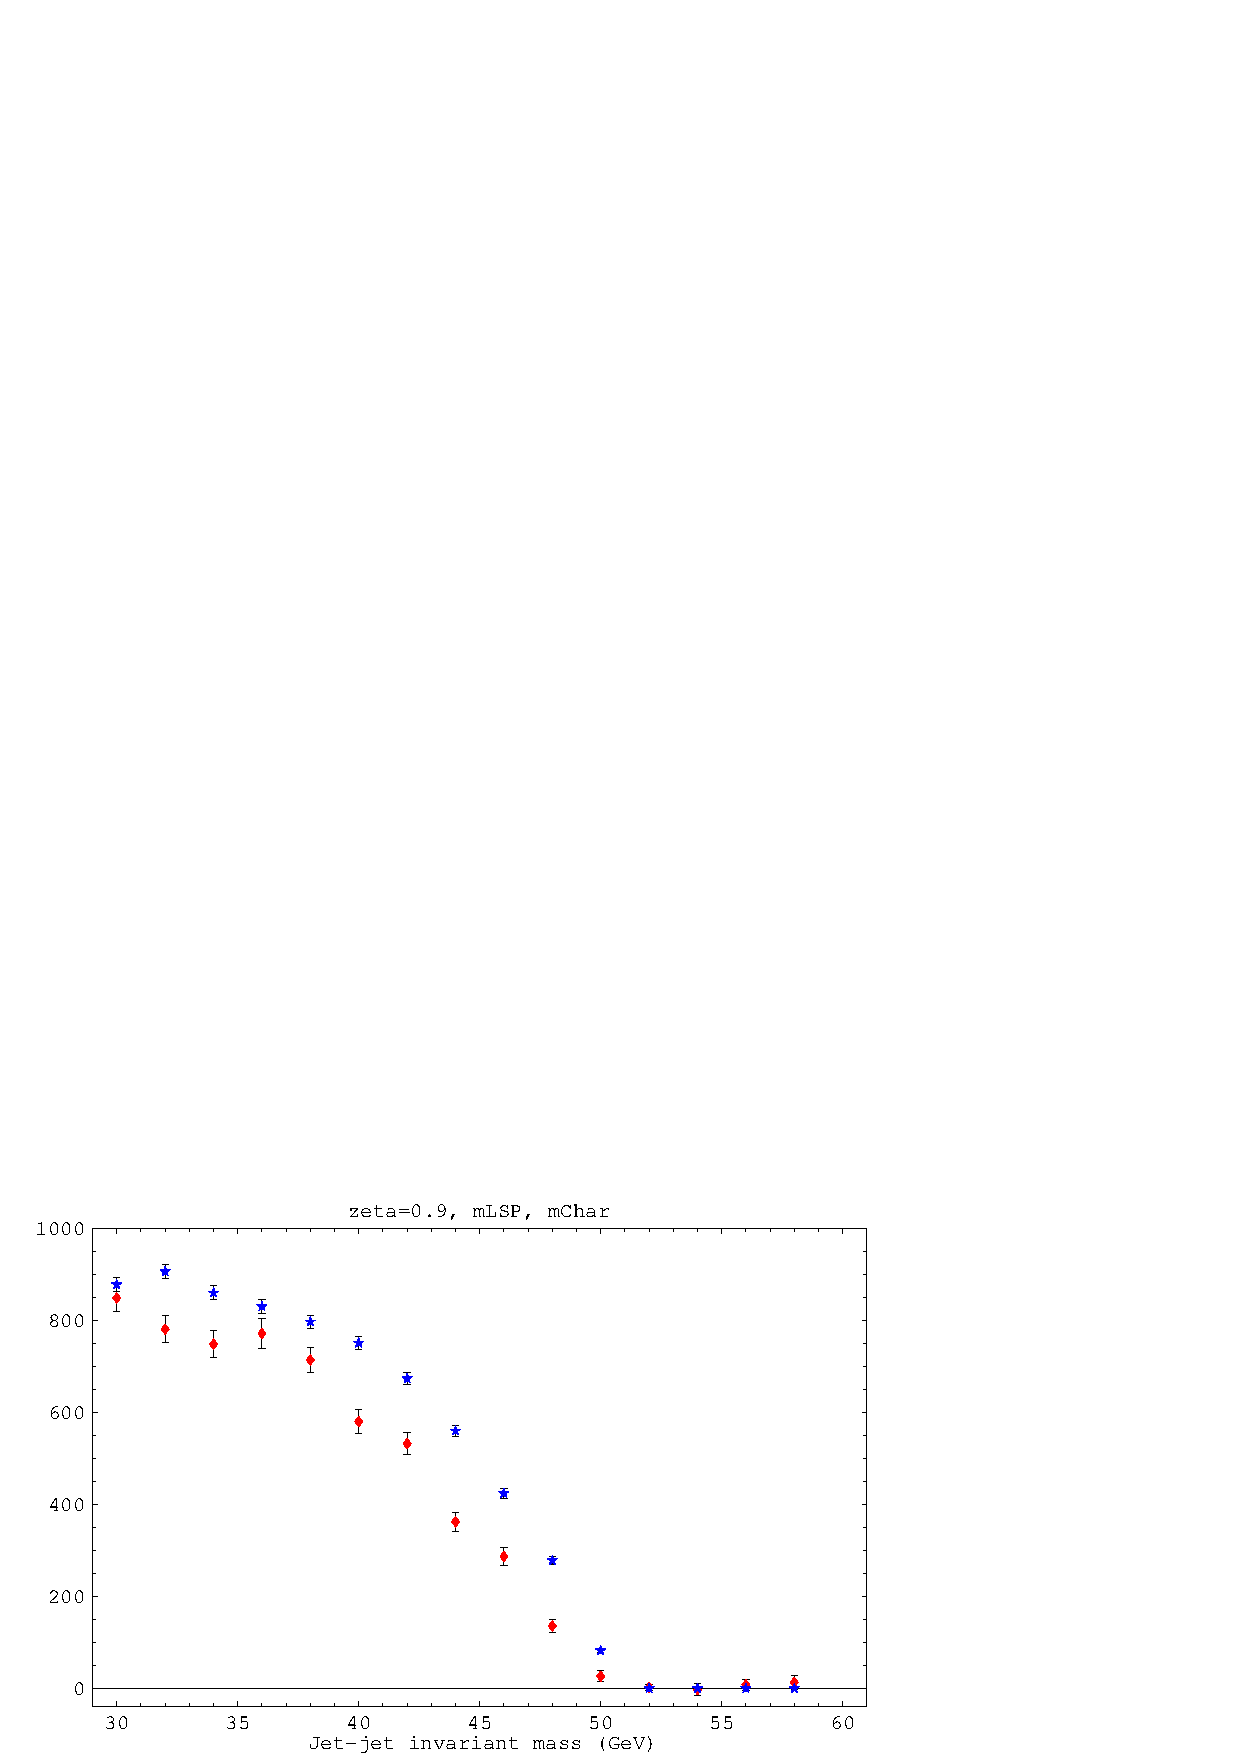
\includegraphics[width=0.5\linewidth]{fakeit_mass.pdf}

\vfill

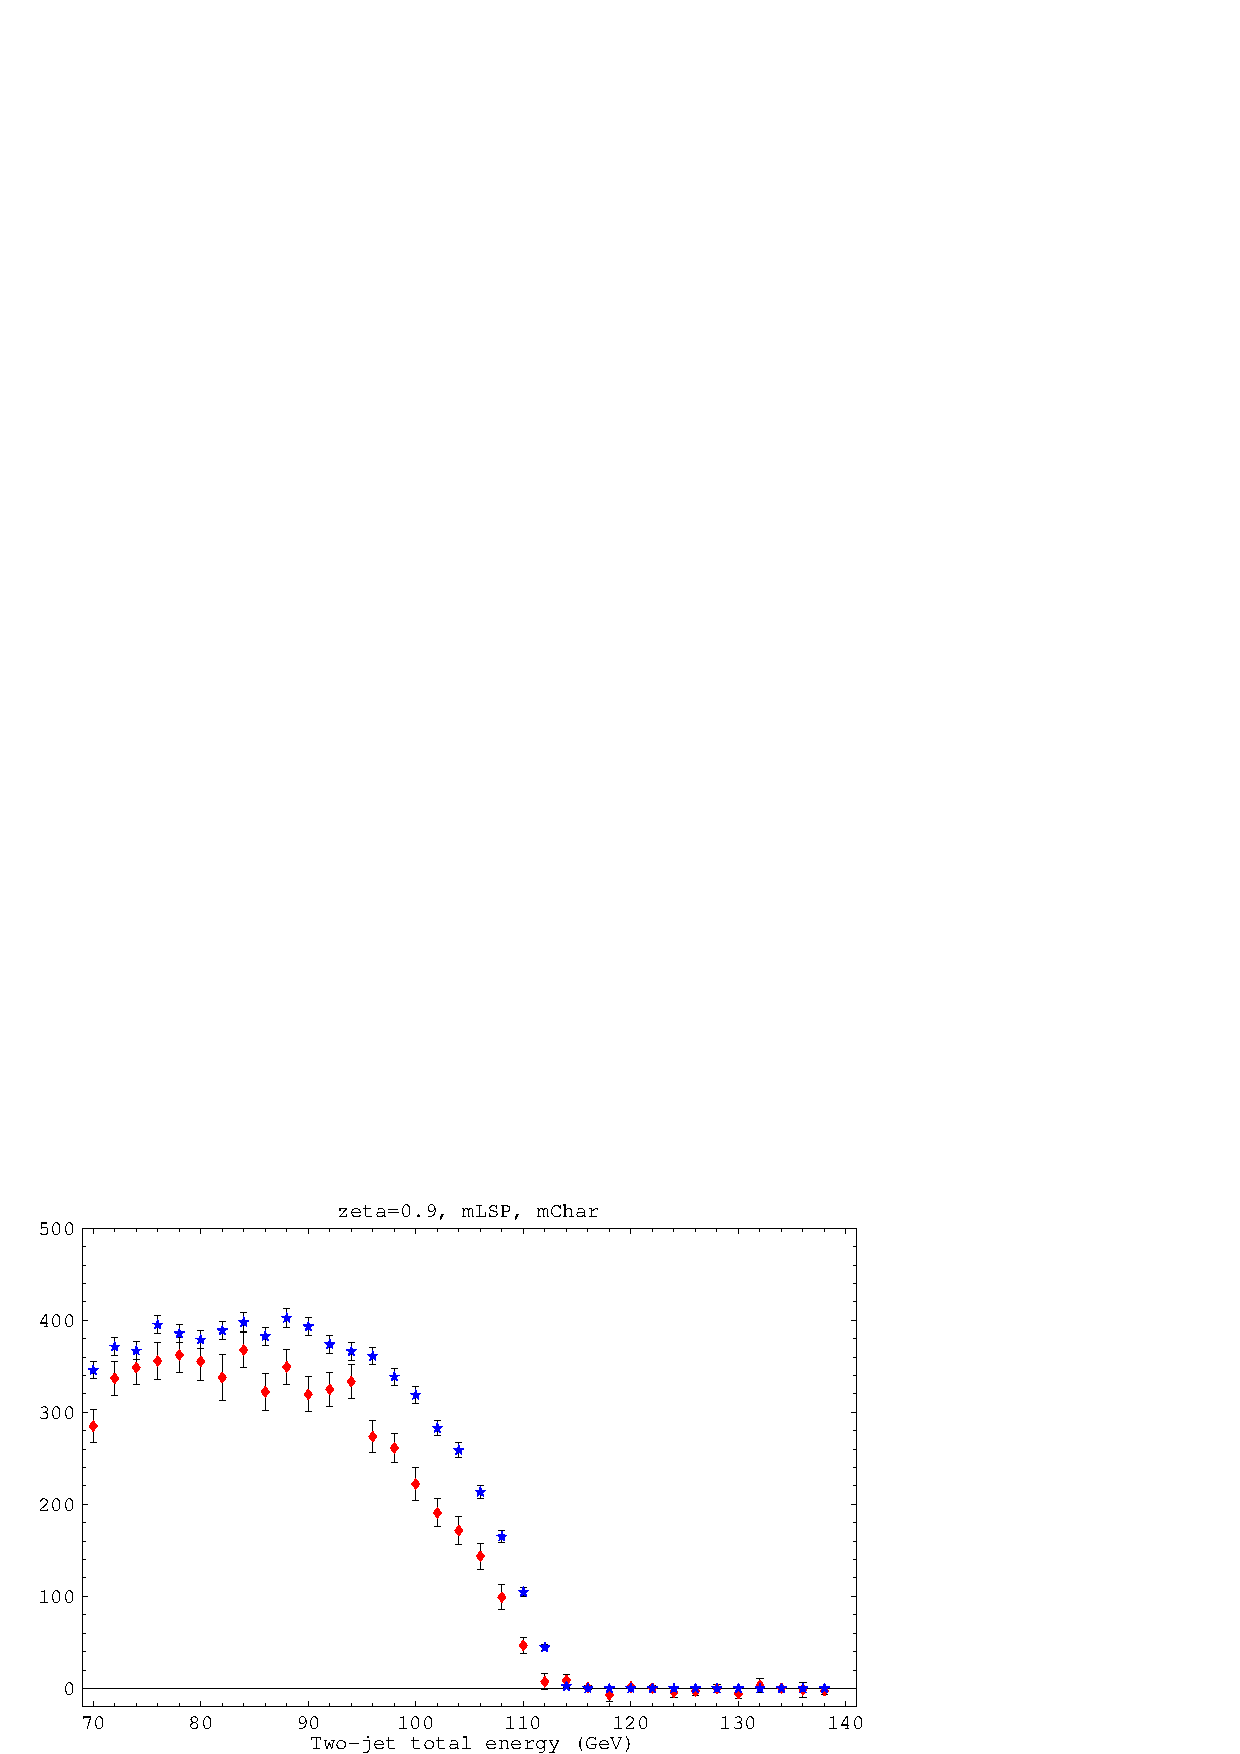
\includegraphics[width=0.5\linewidth]{fakeit_energy.pdf}

\pagebreak

What came out?

\vfill

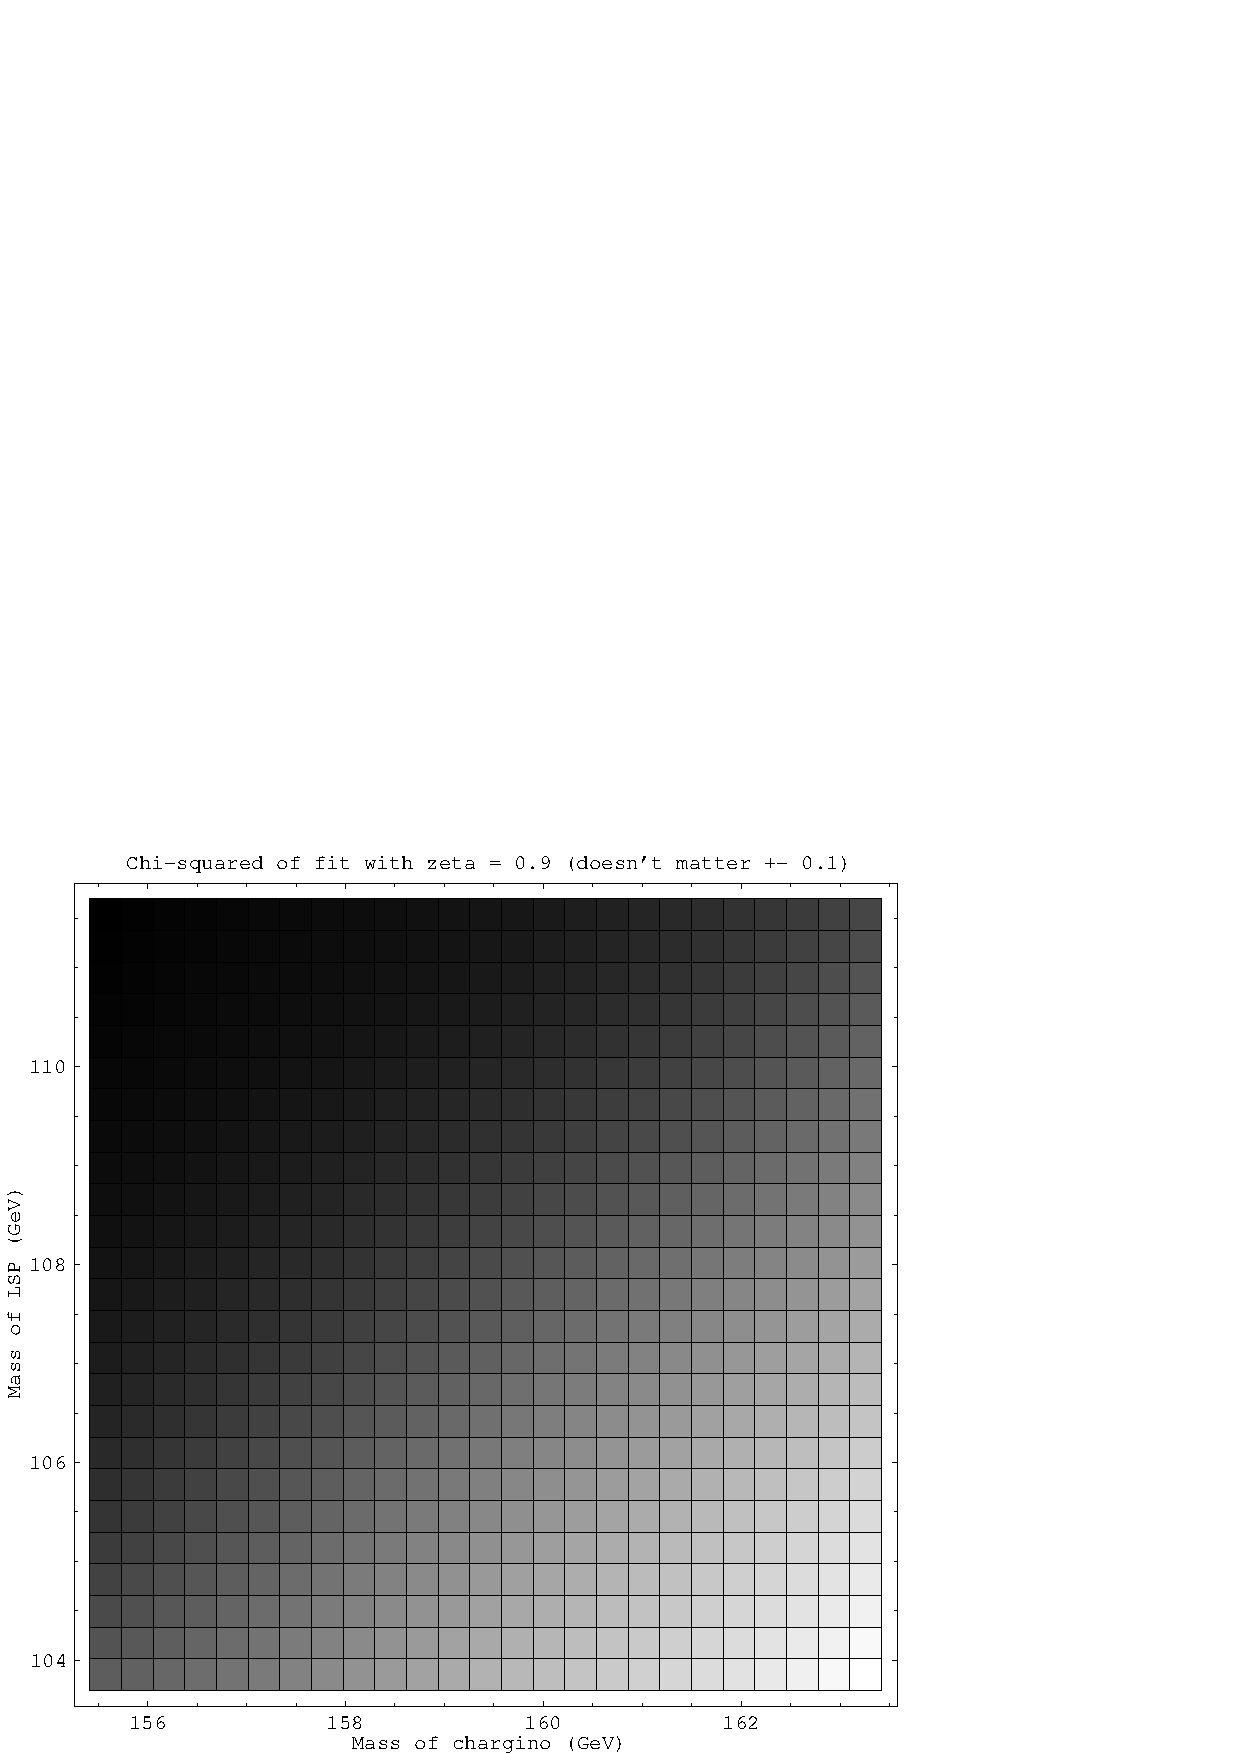
\includegraphics[width=0.7\linewidth]{fakeit_chisquare.pdf}

\pagebreak

What came out?

\vfill

\includegraphics[width=0.5\linewidth]{fakeit_plus4mass.pdf}

\vfill

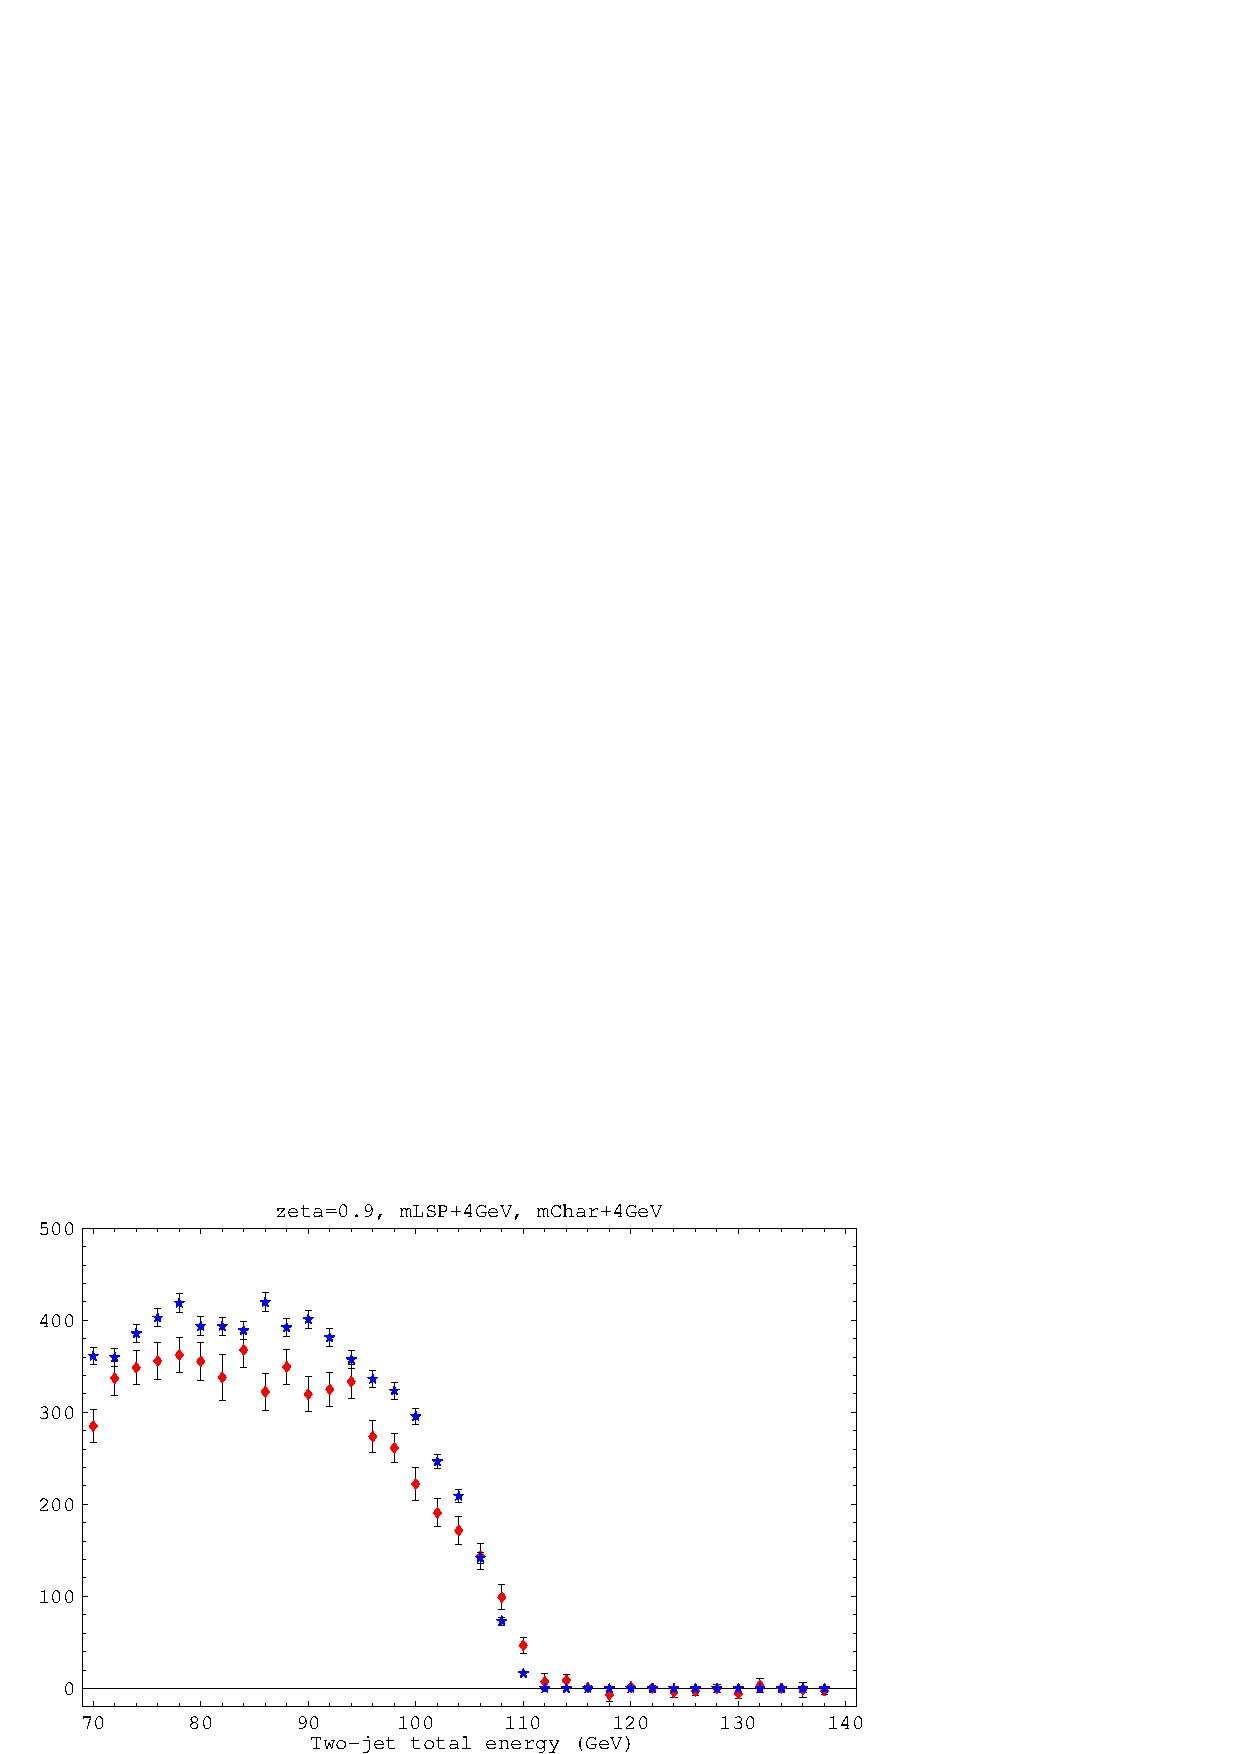
\includegraphics[width=0.5\linewidth]{fakeit_plus4energy.pdf}

\pagebreak

\mbox{ }

\vfill

What to do?

\vfill

Current thoughts: I'm starting to get hung up on detector issues that
are already in the Monte Carlo.  Maybe the following will be sufficient:

\vspace{1 cm}

\begin{itemize}

  \item Use generator-level quantities with no cuts, but reduce the
  statistics to after-cuts levels

  \item Remove detector effects from my model, of course!

  \item Claim that this perfect fit will give the right statistical
  uncertainty, but not systematic errors like understanding your
  detector--- it's a best-case

\end{itemize}

\vfill

\mbox{ }

\vfill

\end{document}
